\documentclass{standalone}
\usepackage{tikz}
\usepackage{ctex,siunitx}
\setCJKmainfont{Noto Serif CJK SC}
\usepackage{tkz-euclide}
\usepackage{amsmath}
\usetikzlibrary{patterns, calc,3d}
\usetikzlibrary {decorations.pathmorphing,decorations.pathreplacing,decorations.shapes}
\begin{document}
\small
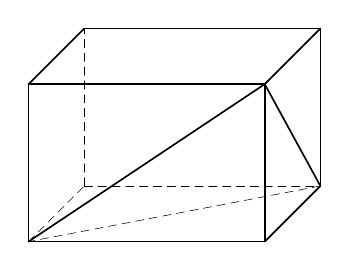
\begin{tikzpicture}[>=latex,scale=1.0]
  \tkzDefPoints{0/0/A,3/0/B,3/2/C,0/2/D,0.707/0.707/A'}
  \tkzDefPointsBy[translation=from A to A'](B,C,D){B',C',D'}
  \tkzDrawPolygon[semithick](A,B,C,D)
  \tkzDrawSegments[semithick](D,D' C,C' B,B' D',C' C',B' C,B' A,C)
  \tkzDrawSegments[densely dashed](A,A' A',B' A',D' B',A)
\end{tikzpicture}
\end{document}